\documentclass[aspectratio=169]{beamer}

\usepackage{tikz}
\usepackage[T1]{fontenc}
\usepackage{newunicodechar}
\usepackage{listings}
\usepackage{comment}
\usepackage{amsmath}
\usepackage[]{graphicx}
\usepackage{subfig}
\usepackage{marvosym}
\usepackage{hyperref}
\usetikzlibrary{positioning}
\usetheme{ulisse}

\definecolor{red2}{HTML}{ED4F4F}

\usepackage{hyperref} % link color
\hypersetup{
    colorlinks=true,
    linkcolor=black,
    urlcolor=red2,
}

\title{Network Security -- Basi e cenni teorici}
\author{Karina Chichifoi (@TryKatChup)}
\date{\today}

\begin{document}
 	\maketitle

	% Intro
	\begin{frame}
		\frametitle{NetSec? Cos?}
		La sicurezza della rete consiste nell'insieme di strategie, procedure e tecnologie finalizzate a proteggere la rete dagli accessi non autorizzati da potenziali danni.\\

		Una delle principali priorità della sicurezza di rete consiste nel controllare l'accesso e impedire che queste minacce riescano a penetrare e a diffondersi al suo interno.\\
	\end{frame}

	\begin{frame}
		\frametitle{NetSec alla CyberChallenge (1/2)}
	    Nel nostro particolare caso sarà molto utile per le competizioni di tipo A/D, dato che dovremmo mantenere sicura la nostra infrastruttura, capire il tipo di traffico in ingresso e uscita, ed evitare intrusioni e il propagarsi di eventuali attacchi.
        \begin{figure}
            \centering
            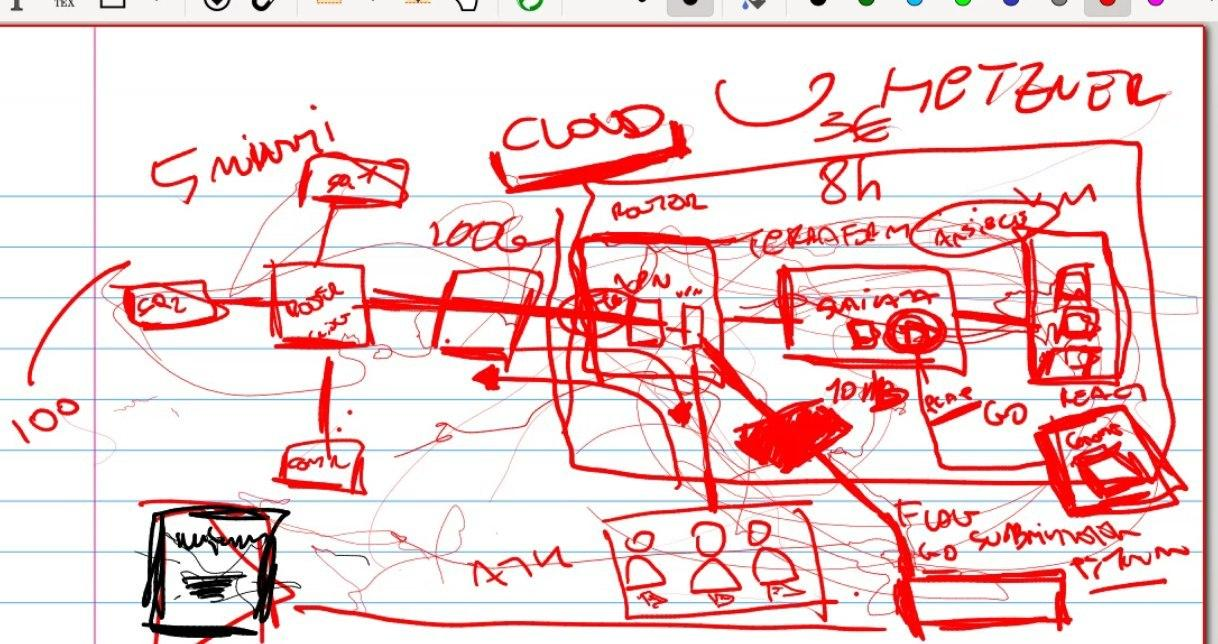
\includegraphics[scale=.3]{img/ctf-infra.jpg}
            \label{fig:infra}
        \end{figure}
	\end{frame} 
    
    \begin{frame}
        \frametitle{NetSec alla CyberChallenge (2/2)}
        \begin{minipage}{\linewidth}
            \centering
            \begin{minipage}{0.45\linewidth}
                \begin{figure}[H]
                \captionsetup{labelfont={color=red2}}
                  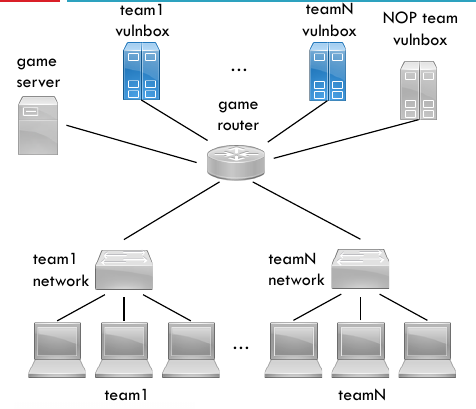
\includegraphics[width=0.88\linewidth]{img/infra-CC.png}
                  \caption{Infrastruttura CC}
                \end{figure}
            \end{minipage}
            \hspace{0.05\linewidth}
            \begin{minipage}{0.45\linewidth}
                \begin{figure}[H]
                \captionsetup{labelfont={color=red2}}
                  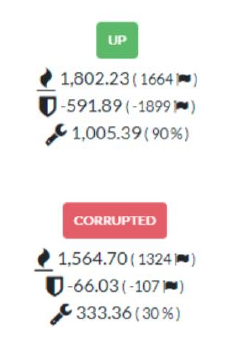
\includegraphics[width=0.5\linewidth]{img/servizi-CC.png}
                  \caption{Stato dei servizi}
                \end{figure}
            \end{minipage}
        \end{minipage}
    \end{frame}
    
    
	\begin{frame}
		\frametitle{Tipologia di reti}
		Suddivisione in base alla dimensione:
		\begin{itemize}
			\item PAN (Personal Area Network): rete ristretta a pochi pc
            \item LAN (Local Area Network): rete locale la cui dimensione può essere relativa a un edificio o a un campus
            \item MAN (Metropolitan Area Network): rete che copre un'intera città
            \item WAN (Wide Area Network): rete che copre uno stato
            \item Internet: copre l'intero pianeta
		\end{itemize}
	\end{frame}
	
	\begin{frame}
    	\frametitle{Sistemi aperti}
        Per sistemi aperti intendiamo una rete di calcolatori in cui qualunque calcolatore o applicazione comunica con qualunque calcolatore o applicazione mediante qualunque rete.
        È importante quindi:
        \begin{itemize}
            \item introdurre regole comuni per lo scambio delle informazioni
            \item utilizzare standard \MVRightarrow{} dispositivi diversi riescono a comunicare
        \end{itemize}
        \vskip 0.3cm
        Da qui nasce OSI (1978), un'architettura a strati.
    \end{frame}
 
    \begin{frame}
    	\frametitle{OSI}
		Lo scopo di OSI è:
		\begin{itemize}
		    \item Scomporre il problema in sottoproblemi più semplici da trattare
		    \item Rendere i vari moduli indipendenti tra loro
		    \item Potere consentire a diversi costruttori di realizzare servizi e interfacce
		\end{itemize}
    \end{frame}
    
    \begin{frame}
        \frametitle{Qualche definizione}
        \begin{itemize}
            \item I servizi sono ciò che viene fornito da uno specifico strato
            \item I protocolli sono il come un certo servizio viene fornito da uno strato. Un protocollo consente a due entità dello stesso livello di potere comunicare tra loro, comprendendo quello che si sta trasmettendo
            \item Un'interfaccia consente di avere regole di dialogo tra entità di livelli adiacenti
            \item L'unità dell'informazione di ciascun livello viene chiamata Protocol Data Unit (PDU)
        \end{itemize}
    \end{frame}

    \begin{frame}
        \frametitle{Protocol Data Unit}
        Ciascun livello inoltre aggiunge all'unità di informazione un header o un footer. Quando l'informazione arriva a destinazione, ciascun livello estrae l'header utile per il suo livello, e passa il resto dell'informazione ai livelli superiori.
        \begin{figure}
            \centering
            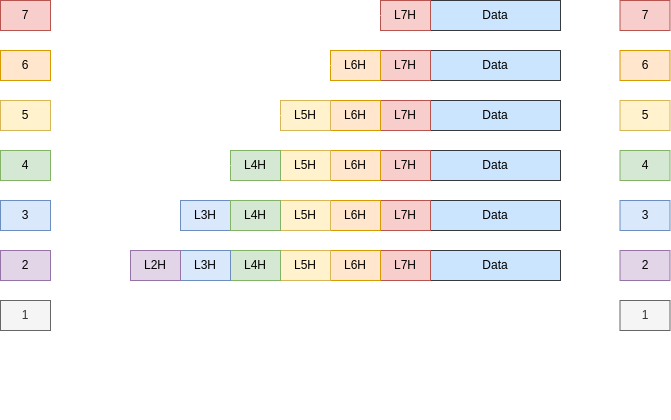
\includegraphics[width=0.55\linewidth]{img/protocol-data-unit.png}
            \label{pdu}
        \end{figure}
    \end{frame}
    
    \begin{frame}
        \frametitle{ISO/OSI}
        \begin{tikzpicture}[overlay,remember picture]
            \node[anchor=south east,xshift=-15pt,yshift=40pt]
              at (current page.south east) {
                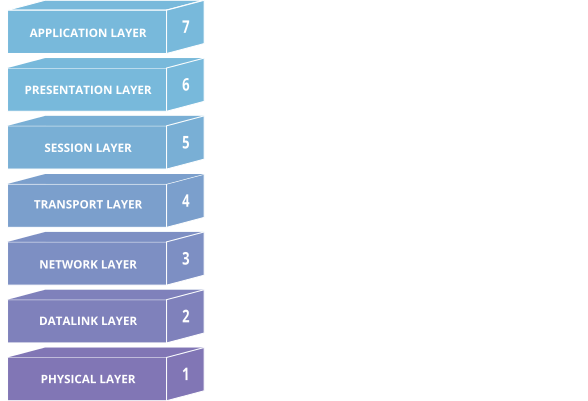
\includegraphics[width=0.55\linewidth]{img/osi.png}
              };
        \end{tikzpicture}%
        In ISO/OSI si hanno 7 strati:
        \begin{itemize}
            \item I primi 3 sono detti lower,\\o network oriented layers
            \item Gli strati 5,6,7 sono detti upper\\o application oriented layers
            \item Lo strato 4 fa da raccordo tra\\upper e lower layers
            \item Gli strati dal 4 in su operano\\invece solo end-to-end
        \end{itemize}
    \end{frame}
    
    \begin{frame}
        \frametitle{Livello 1: Physical layer}
        \begin{tikzpicture}[overlay,remember picture]
            \node[anchor=south east,xshift=-15pt,yshift=20pt]
              at (current page.south east) {
                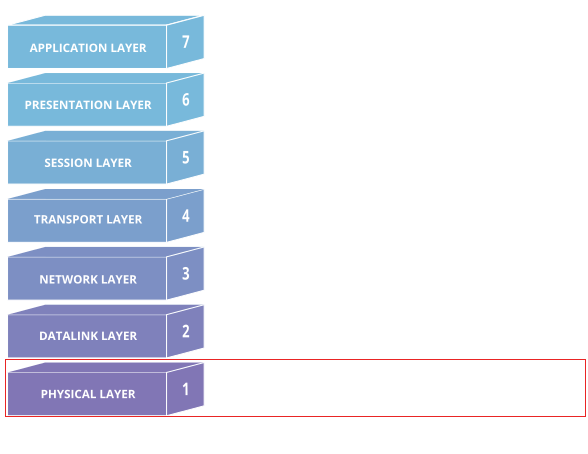
\includegraphics[width=0.55\linewidth]{img/physical_layer.png}
              };
        \end{tikzpicture}%
        Consente di trasmettere un flusso di\\dati attraverso un collegamento fisico,\\occupandosi della forma e dei livelli\\di tensione del segnale.
        \begin{itemize}
            \item Unità dati: bit
            \item Tecnologie: bluetooth, fibra ottica,\\cavo di rame
        \end{itemize}
    \end{frame}
    
    \begin{frame}
        \frametitle{Livello 2: Data link layer}
        \begin{tikzpicture}[overlay,remember picture]
            \node[anchor=south east,xshift=-15pt,yshift=20pt]
              at (current page.south east) {
                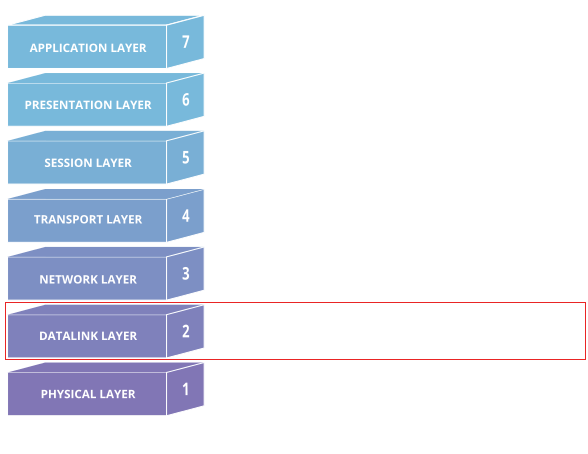
\includegraphics[width=0.55\linewidth]{img/datalink_layer.png}
              };
        \end{tikzpicture}%
        Consente un trasferimento affidabile di\\dati a livello fisico.
        \vskip 0.3cm
        Effettua anche un controllo degli errori\\ e perdite di segnale.
        \begin{itemize}
            \item Unità dati: frame
            \item Protocolli: Ethernet, Wi-Fi
        \end{itemize}
    \end{frame}
    
    \begin{frame}
        \frametitle{Livello 3: Network layer}
        \begin{tikzpicture}[overlay,remember picture]
            \node[anchor=south east,xshift=-15pt,yshift=20pt]
              at (current page.south east) {
                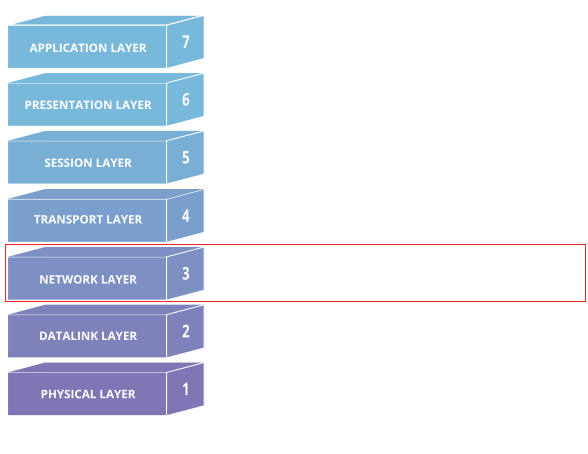
\includegraphics[width=0.55\linewidth]{img/network_layer.png}
              };
        \end{tikzpicture}%
        Rende i livelli indipendenti dai\\meccanismi e dalle tecnologie usate\\per la connessione.
        \vskip 0.3cm
        Lo scopo di questo livello è di far\\giungere le unità di informazioni\\(pacchetti) al destinatario, scegliendo\\il percorso attraverso la rete.\vskip 0.3cm
        Si occupa del routing, consentendo il\\corretto instradamento dei pacchetti\\verso la giusta destinazione.
        \begin{itemize}
            \item Unità dati: pacchetto
            \item Protocolli: IP
        \end{itemize}
    \end{frame}
    
    \begin{frame}
        \frametitle{Livello 4: Transport layer}
        \begin{tikzpicture}[overlay,remember picture]
            \node[anchor=south east,xshift=-15pt,yshift=20pt]
              at (current page.south east) {
                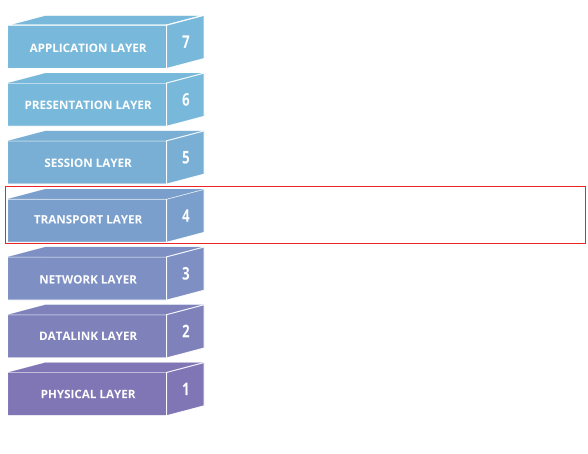
\includegraphics[width=0.55\linewidth]{img/transport_layer.png}
              };
        \end{tikzpicture}%
        Consente un trasferimento dati\\trasparente e affidabile, effettuando\\un controllo degli errori e flusso\\tra due host.
        \vskip 0.3cm
        Il suo scopo è di fornire un canale\\sicuro end-to-end, svincolando gli\\strati superiori dai problemi di rete.

        \begin{itemize}
            \item Unità dati: segmenti
            \item Protocolli: TCP, UDP
        \end{itemize}
    \end{frame}
    
    \begin{frame}
      \frametitle{Livello 5: Session Layer}%
      
      \begin{tikzpicture}[overlay,remember picture]
            \node[anchor=south east,xshift=-15pt,yshift=20pt]
              at (current page.south east) {
                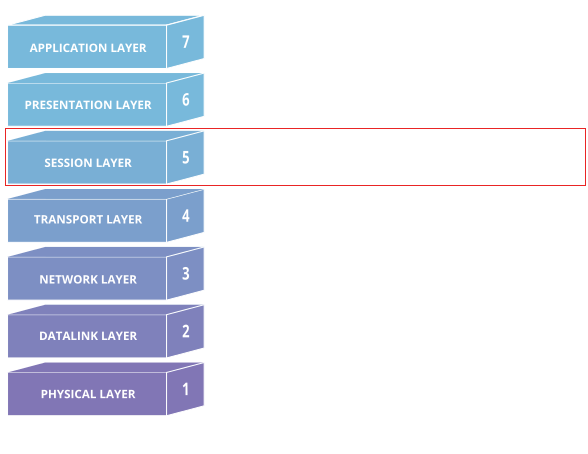
\includegraphics[width=0.55\linewidth]{img/session_layer.png}
              };
      \end{tikzpicture}%
      
      Consente di stabilire, gestire e\\ terminare sessioni di comunicazione\\tra applicazioni.
      \vskip 0.3cm
      Vengono introdotti anche dei punti di\\ sincronizzazione (token) e vengono\\inseriti checkpoint, in modo da ridurre\\la quantità di dati da ritrasmettere\\in caso di gravi malfunzionamenti.
        \begin{itemize}
            \item Protocolli: SOCKS, NetBIOS
        \end{itemize}
    \end{frame}
    
    \begin{frame}
      \frametitle{Livello 6: Presentation layer}%
      
      \begin{tikzpicture}[overlay,remember picture]
            \node[anchor=south east,xshift=-15pt,yshift=20pt]
              at (current page.south east) {
                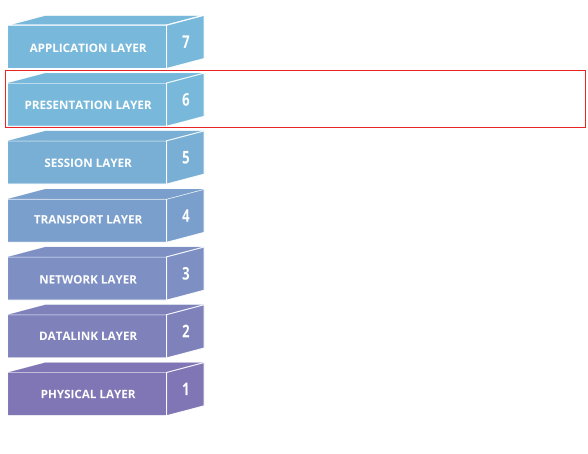
\includegraphics[width=0.55\linewidth]{img/presentation_layer.png}
              };
      \end{tikzpicture}%
      
      Si occupa della trasformazione\\ dei dati in un formato standard,\\ e offre servizi come la compressione\\ e cifratura.
      \begin{itemize}
            \item Protocolli: PGP, MIME, ASCII
       \end{itemize}
    \end{frame}
    
    \begin{frame}
      \frametitle{Livello 7: Application Layer}%
      
      \begin{tikzpicture}[overlay,remember picture]
            \node[anchor=south east,xshift=-15pt,yshift=20pt]
              at (current page.south east) {
                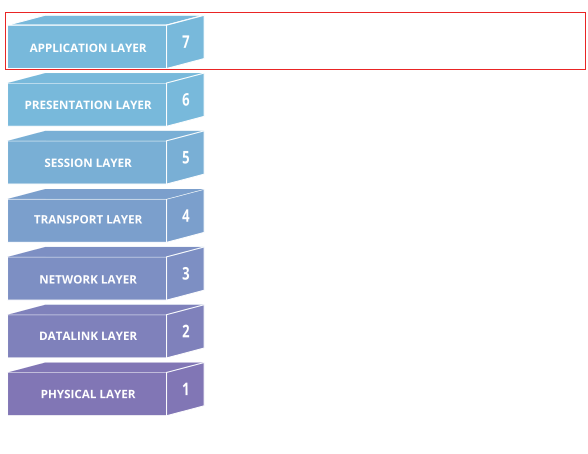
\includegraphics[width=0.55\linewidth]{img/application_layer.png}
              };
      \end{tikzpicture}%
      
      Fornisce servizi per i processi\\delle applicazioni.
        \begin{itemize}
            \item Protocolli: DHCP, DNS, LDAP,\\SSH, HTTP
        \end{itemize}
    \end{frame}
    
    \begin{frame}
      \frametitle{TCP/IP}%
      
      \begin{tikzpicture}[overlay,remember picture]
        \node[anchor=south east,xshift=10pt,yshift=35pt]
          at (current page.south east) {
            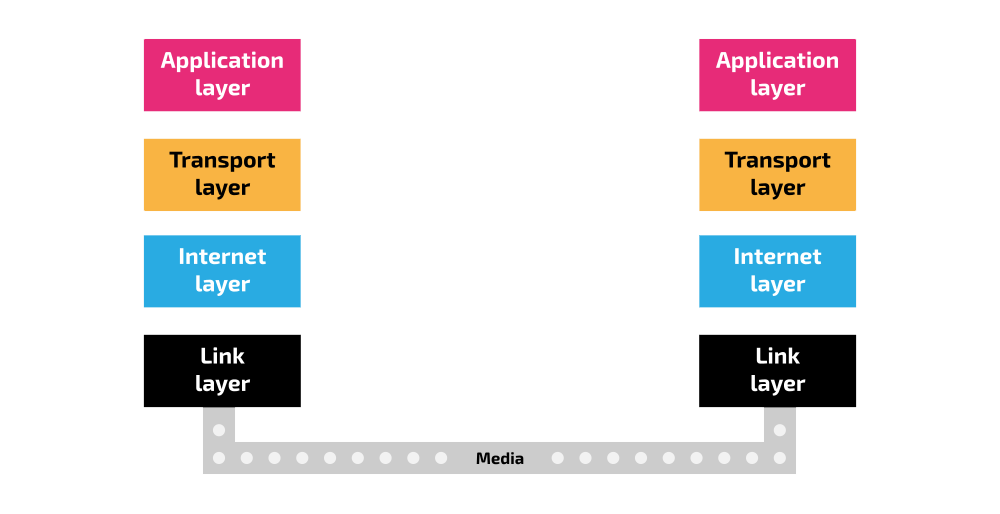
\includegraphics[width=0.7\linewidth]{img/tcp_ip.png}
          };
      \end{tikzpicture}%
      
      ISO/OSI è stato creato nel 1978\\è evoluto come modello teorico;\\ al contrario TCP/IP risulta un modello\\ pratico, utilizzato normalmente per le\\ implementazioni delle funzioni di rete.
    \end{frame}
    
    \begin{frame}
        \frametitle{MAC Address}
        Ciascuna scheda di rete di un dispositivo è identificata da un MAC Address, ovvero un indirizzo a 6 byte strutturato nel seguente modo:
        \begin{center}
            00:50:FC:A0:67:2C
        \end{center}
        Dove:
        \begin{itemize}
            \item I primi 3 ottetti (ovvero i primi 24 bit) dipendono unicamente dal produttore della scheda di rete. In particolare, se si considera il primo byte e si guarda l'ultimo bit si ha:
            \begin{itemize}
                \setbeamercolor{itemize subitem}{fg=red2}
                \setbeamertemplate{itemize subitem}[square]
                \item Multicast se bit = 1
                \item Unicast se bit = 0
            \end{itemize}
            \item I successivi 3 ottetti dipendono dal numero di serie della scheda di rete stessa:
            \begin{itemize}
                \item Si hanno $2^{48}$ (cioè 281.474.976.710.656) indirizzi MAC possibili, che è un numero che è impossibile raggiungere prima che le schede di rete cambino standard
            \end{itemize}
        \end{itemize}
    \end{frame}
    
    \begin{frame}
        \frametitle{Mac Address: struttura}
        \begin{figure}
            \centering
            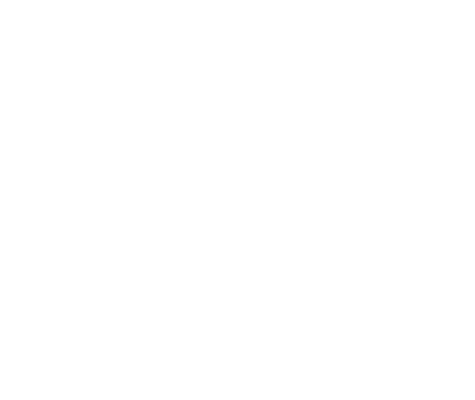
\includegraphics[width= 0.5\linewidth]{img/MAC-48_Address.png}
        \end{figure}
    \end{frame}
    
    \begin{frame}
        \frametitle{Destinatari}%
        
        \begin{tikzpicture}[overlay,remember picture]
        \node[anchor=south east,xshift=-30pt,yshift=60pt]
          at (current page.south east) {
            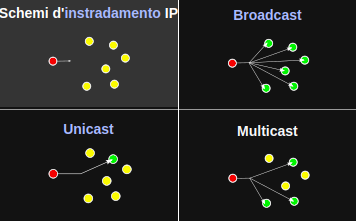
\includegraphics[width=0.40\linewidth]{img/unicast_multicast.png}
          };
        \end{tikzpicture}%
        
        Normalmente un messaggio può essere\\ inviato in:
        \begin{itemize}
            \item Unicast: un dispositivo invia l'informazione\\ a  un solo dispositivo
            \item Multicast: un' informazione viene inviata\\ a più dispositivi finali
            \item Broadcast: l'informazione viene inviata\\ contemporaneamente a tutti i dispositivi\\ presenti nella rete (\texttt{FF:FF:FF:FF:FF:FF})
        \end{itemize}
    \end{frame}
    
    \begin{frame}
        \frametitle{MAC Spoofing}
        Utile per motivi di:
        \begin{itemize}
            \item Privacy
            \item Interoperabilità
        \end{itemize}
        La randomizzazione dell'indirizzo MAC della scheda WIFI è abilitata di default su:
        \begin{itemize}
            \item Android >=8
            \item iOS >=14
        \end{itemize}
        Per abilitarla su Arch: \href{https://wiki.archlinux.org/title/MAC_address_spoofing}{link}\\
        Per abilitarla su Windows: \href{https://support.microsoft.com/en-us/windows/how-to-use-random-hardware-addresses-in-windows-ac58de34-35fc-31ff-c650-823fc48eb1bc}{link}
    \end{frame}
    
    \begin{frame}
        \frametitle{IP}
        Protocollo a livello di rete: 
        \begin{itemize}
            \item Connectionless: assenza di richiesta di connessione \MVRightarrow{} non c'è garanzia che il singolo pacchetto sia stato consegnato, né che sia stato consegnato nell'ordine corretto.
            \item Non affidabile: i datagram possono essere persi o danneggiati durante il tragitto oppure potrebbero arrivare in ordine sparso a destinazione.
        \end{itemize}
    \end{frame}
    
    \begin{frame}
        \frametitle{Router for newbies}
        Il router è il principale attore del compito di instradamento dei dati.
        È un vero e proprio calcolatore con una CPU e una RAM.
        \begin{figure}
            \centering
            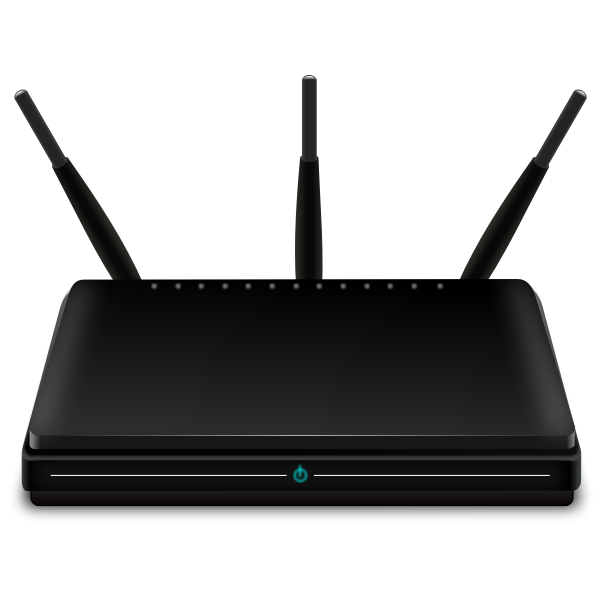
\includegraphics[width=0.30\linewidth]{img/wireless-router.png}
            \label{fig:router}
        \end{figure}
    \end{frame}
    
    \begin{frame}
        \frametitle{Tabella di routing}
        La tabella di routing contiene le rotte verso altri router e il loro costo.\\
        Il costo, o metrica, sono informazioni basate sulla larghezza di banda, numero di hop (nodi della rete), il ritardo, carico, Maximum Transmission Unit, affidabilità della comunicazione.\vskip 0.3cm
        
        I protocolli di routing sono un insieme di norme che regolamentano la comunicazione tra due router.
        Forniscono informazioni utili sulle rotte più comode da utilizzare attraverso le quali inviare i pacchetti.
    \end{frame}
     
    \begin{frame}
        \frametitle{IPv4}
        \begin{center}
            \texttt{137.204.150.24}
        \end{center}
        \begin{itemize}
            \item Indirizzi composti da 32 bit
            \item Si hanno pertanto $2^{32}$ indirizzi IPv4 possibili (4,294,967,296)
            \item Un indirizzo IP definisce in modo univoco un'interfaccia di rete connessa ad un LAN o WAN
            \item Esistono anche i multi-homed host, ovvero host con due o più interfacce di rete che usa più indirizzi IP
            \item Un router che collega N reti ha almeno N distinti indirizzi IP, uno per ogni interfaccia di rete
        \end{itemize}
    \end{frame}
    
    \begin{frame}
        \frametitle{Classi IP}
        Abbiamo ben 5 classi di indirizzi IP:
        \begin{itemize}
            \item Classe A: da \texttt{0.0.0.0} a \texttt{127.255.255.255}
            \item Classe B: da \texttt{128.0.0.0} a \texttt{191.255.255.255}
            \item Classe C: da \texttt{192.0.0.0} a \texttt{223.255.255.255}
            \item Classe D: da \texttt{224.0.0.0} a \texttt{239.255.255.255}
            \item Classe E: da \texttt{240.0.0.0} a \texttt{255.255.255.255}
        \end{itemize}
    
    \end{frame}
    
    \begin{frame}
        \frametitle{Classi IP}
        Esistono anche una serie di indirizzi riservati (RFC 1700, 3927)
        \begin{itemize}
            \item \texttt{0.0.0.0} indica l'host corrente senza specificarne l'indirizzo
            \item \texttt{0.x.y.z} indica un certo Host-ID sulla rete corrente senza specificare il Net-ID
            \item \texttt{255.255.255.255} è l'indirizzo di limited broadcast
            \item \texttt{127.x.y.z} è il loopback, che redirige i datagrammi agli strati superiori
            \item \texttt{169.254.x.y} riservati per l'autoconfigurazione degli host
        \end{itemize}
    \end{frame}
        
    \begin{frame}
        \frametitle{CIDR}
        In molti casi una rete di classe \texttt{A} o \texttt{B} è troppo grande (molti indirizzi inutilizzati) e una di classe \texttt{C} troppo piccola.\vskip 0.3cm
    
        Indirizzamento IP più flessibile senza l'uso delle classi: pertanto adesso si utilizza CIDR (Classless Inter-Domain Routing)
    \end{frame}
    
    \begin{frame}
        \frametitle{Suddivisione di un indirizzo IP}
        Un indirizzo IP è diviso in due parti:
        \begin{itemize}
            \item Network-ID che identifica la rete (prefisso)
            \item Host-ID che identifica l'host all'interno della rete (suffisso)
        \end{itemize}
        La suddivisione è indicata dalla netmask, una sequenza di 4 byte associata all'indirizzo, in cui
        \begin{itemize}
            \item i bit a 1 corrispondono ai bit dedicati al Network-ID
            \item i bit a 0 corrispondono ai bit dedicati al Host-ID
        \end{itemize}
    \end{frame}
    
    \begin{frame}
        \frametitle{Netmask}
        \begin{itemize}
            \item Composta da 32 bit
            \item Specifica il numero massimo di host disponibili in una rete
            \item Può indicare per quali dispositivi si applica una specifica regola (ad esempio con iptables)
        \end{itemize}
        Per definizione, una netmask ha sempre tutti i bit a 1 a sinistra e tutti quelli a 0 a destra.
        \\
        Non esistono netmask con degli 0 tra gli 1.
        \begin{itemize}
            \item \texttt{11111011.11011111.11100000.00010000} non è valida!
        \end{itemize}
    \end{frame}
    
    \begin{frame}
        \frametitle{Possibili valori della netmask}
        Di conseguenza, i singoli byte di una netmask non possono assumere tutti i 256 valori possibili, ma solo 9:
        \vskip 0.5cm
        \begin{minipage}{\linewidth}
            \centering
            \begin{minipage}{0.45\linewidth}
                \begin{itemize}
                    \item \texttt{00000000} = 0
                    \item \texttt{10000000} = 128
                    \item \texttt{11000000} = 192
                    \item \texttt{11100000} = 224
                    \item \texttt{11110000} = 240
                \end{itemize}
            \end{minipage}
            \hspace{0.05\linewidth}
            \begin{minipage}{0.45\linewidth}
                \begin{itemize}
                    \item \texttt{11111000} = 248
                    \item \texttt{11111100} = 252
                    \item \texttt{11111110} = 254
                    \item \texttt{11111111} = 255
                \end{itemize}
            \end{minipage}
        \end{minipage}
    \end{frame}
    
    \begin{frame}
        \frametitle{Struttura di un indirizzo IP}
        \begin{figure}
            \centering
            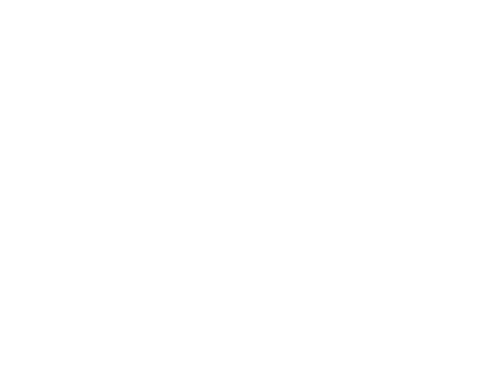
\includegraphics[width= 0.68\linewidth]{img/networkid.png}
        \end{figure}
    \end{frame}
    
    \begin{frame}
        \frametitle{Struttura di una netmask}
        \begin{tikzpicture}[overlay,remember picture]
        \node[anchor=south east,xshift=-20pt,yshift=35pt]
        at (current page.south east) {
        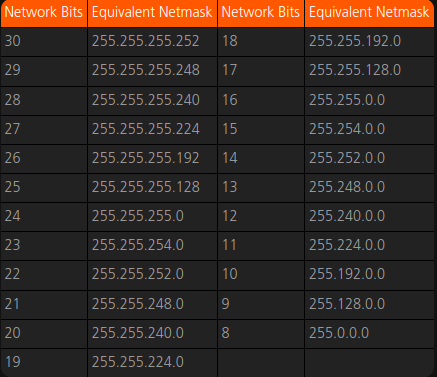
\includegraphics[width=0.5\linewidth]{img/table-netmask.png}
        };
        \end{tikzpicture}%
        
        Si hanno quindi 4 byte, ognuno\\dei quali con i valori visti in precedenza.\vskip 0.3cm
        La netmask si può specificare\\alla fine di un indirizzo IP nel seguente\\modo:
        \texttt{192.168.1.0/24}\vskip 0.3cm
        Per testare le varie configurazioni:
        \begin{itemize}
            \item comando \texttt{ipcalc}
            \item questo sito: \href{http://jodies.de/ipcalc}{link}
        \end{itemize}
        
    \end{frame}
    
    \begin{frame}
        \frametitle{Esempio 1}
        Rete IP a disposizione: \texttt{192.168.1.0/24}\\
        LAN A ha 50 host:
        \begin{itemize}
            \item mi basta una sottorete da 62 indirizzi host
            \item \texttt{192.168.1.0/26} è un Net-ID valido
        \end{itemize}
        LAN B ha 100 host:
        \begin{itemize}
            \item mi basta una sottorete da 126 indirizzi host
            \item \texttt{192.168.1.64/25} NON è un Net-ID valido
            \item \texttt{64 = 01000000}
            \item \texttt{192.168.1.128/25} è un Net-ID valido
            \item \texttt{128 = 10000000}
        \end{itemize}
    \end{frame}
    
    \begin{frame}
        \frametitle{Problematiche di IPv4}
        Ci sono diverse problematiche relative a IPv4:
        \begin{itemize}
            \item Se un host viene spostato in un'altra rete, il suo indirizzo IP deve cambiare
            \item Occorre automatizzare l'assegnazione della configurazione degli indirizzi IP dei diversi client in una intranet \MVRightarrow{} DHCP
            \item Data l'enorme diffusione di Internet, il numero di indirizzi possibili è troppo basso \MVRightarrow{} utile l'adozione di reti IP private e di tecniche di NAT (Network Address Translation)
        \end{itemize}
    \end{frame}
    
    \begin{frame}
        \frametitle{NAT (Network Address Translation)}
        Consente a più dispositivi di accedere a internet mediante un solo indirizzo IP. Si occupa della traduzione da indirizzi IP pubblici e privati e viceversa.\\
        Indirizzi riservati a reti IP private:
        \begin{itemize}
            \item da \texttt{10.0.0.0} a \texttt{10.255.255.255}
            \item da \texttt{172.16.0.0.0} a \texttt{172.31.255.255} (rete aziendale)
            \item da \texttt{192.168.0.0} a \texttt{192.168.255.255} (rete di casa)
        \end{itemize}
    \end{frame}
    
    \begin{frame}
        \frametitle{DHCP}
        Un server DHCP ha il compito di assegnare ad un dispositivo che si connette alla sua rete il primo indirizzo IP valido disponibile.
        Quando un host collegato ad una LAN o ad una linea vuole usare il DHCP:
        \begin{itemize}
            \item Invia un messaggio \texttt{DHCPDISCOVER} in broadcast
            \item Uno o più Server se presenti rispondono con \texttt{DHCPOFFER}
            \item L'Host ne sceglie uno e gli invia \texttt{DHCPREQUEST} per richiedere la configurazione
            \item Il Server risponde con \texttt{DHCPACK} specificando la configurazione
        \end{itemize}
        È necessario un server DHCP (porta 67 UDP).
    \end{frame}
    
    
    \begin{frame}
        \frametitle{IP Spoofing}
        L'IP spoofing consiste nella creazione di un pacchetto con i source address modificati, in modo da sia nascondere l'identità del mittente, sia eventualmente per impersonificare qualcun altro, o entrambe. 
        
        È una tecnica utilizzata solitamente dai malitenzionati per utilizzare attacchi DOS contro uno specifico dispositivo o infrastruttura.
    \end{frame}
    
    \begin{frame}
        \frametitle{ARP}
        ARP (Address Resolution Protocol) è un protocollo collocato tra il livello 2 e il livello 3 ISO/OSI che consente di ottenere un indirizzo fisico di un nodo, partendo dal suo indirizzo IP.
        \begin{itemize}
            \item Alice vuole sapere l'indirizzo MAC di Bob
            \item A tal scopo, Alice invia un pacchetto broadcast (ARP Request) per richiedere l'indirizzo fisico corrispondente all'IP di Bob
            \item  Tutti gli host della rete ricevono quel pacchetto e solo chi riconosce il proprio indirizzo IP risponde con il proprio indirizzo fisico, ovvero Bob (ARP Reply)
        \end{itemize}
        Viene utilizzata una memoria cache per mantenere le associazioni \{indirizzo IP - indirizzo fisico\} utilizzate.
    \end{frame}
    
    \begin{frame}
        \frametitle{ARP poisoning}
        Sfrutta il mancato meccanismo di autenticazione del protocollo ARP: qualsiasi dispositivo può rispondere a un ARP Request.\\
        L'attaccante invierà delle opportune ARP request modificate, in modo da popolare l'ARP cache con il proprio indirizzo MAC.
        \vskip 0.5cm
        Modalità di attacco:
        \begin{itemize}
            \item Man in the Middle
            \item Denial of Service
        \end{itemize}
    \end{frame}
    
    \begin{frame}
        \frametitle{Come prevenire ARP poisoning?}
        \begin{itemize}
            \item Tabelle ARP statiche
            \item Controllo degli accessi alla rete locale
            \item Suddivisione della rete
            \item Comunicazione cifrata
        \end{itemize}
    \end{frame}
    
    \begin{frame}
        \frametitle{Livello di trasporto: TCP}
        TCP è un protocollo connection-oriented utilizzato nel livello di trasporto e, assieme a Internet Protocol, garantisce affidabilità nella trasmissione dei dati, sfruttando un canale di trasmissione bidirezionale.
        \vskip 0.3cm
        TCP garantisce:
        \begin{itemize}
            \item Comunicazione process to process
            \item Consegna prioritaria di dati (se specificato) su banda limitata
            \item Consegna ordinata dei dati
            \item Controllo di flusso
            \item Controllo di congestione.
        \end{itemize}
    \end{frame}
    
    \begin{frame}
        \frametitle{Three way handshake}
        \begin{tikzpicture}[overlay,remember picture]
        \node[anchor=south east,xshift=-5pt,yshift=55pt]
        at (current page.south east) {
        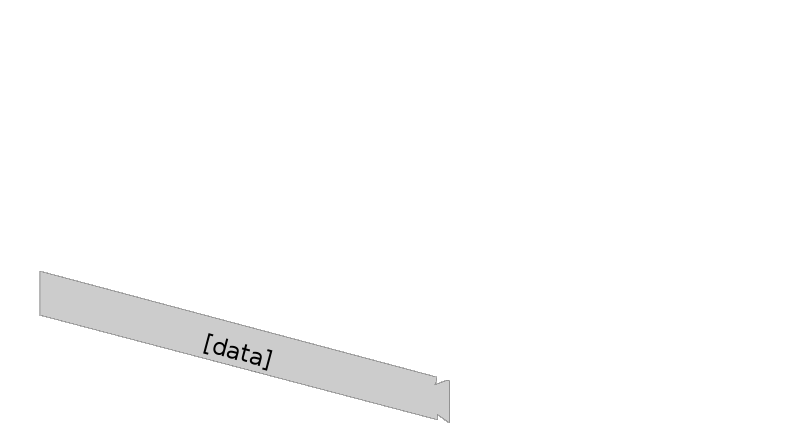
\includegraphics[width=0.55\linewidth]{img/ack.png}
        };
        \end{tikzpicture}%
        Consente di stabilire una connessione\\ affidabile.
        Vengono utilizzati dei valori\\ contenuti nel segmento, \texttt{seq} e \texttt{ack},\\ che consentono sia a mittente che a\\ destinatario di coordinarsi tra loro e di\\ verificare la corretta ricezione.
    \end{frame}
    
    \begin{frame}
        \frametitle{UDP}
        UDP è un protocollo di trasporto a pacchetto a basso costo, utilizzato in combinazione con il protocollo del livello di rete IP.\\
        Fornisce un servizio unreliable e connectionless: i datagrammi possono essere persi, duplicati, consegnati fuori ordine o arrivare in ritardo.\\
        Normalmente utilizzato per gli stream video.
    \end{frame}
    
    \begin{frame}
        \frametitle{TCP vs UDP}
        \begin{tikzpicture}[overlay,remember picture]
        \node[anchor=south east,xshift=-10pt,yshift=20pt]
        at (current page.south east) {
        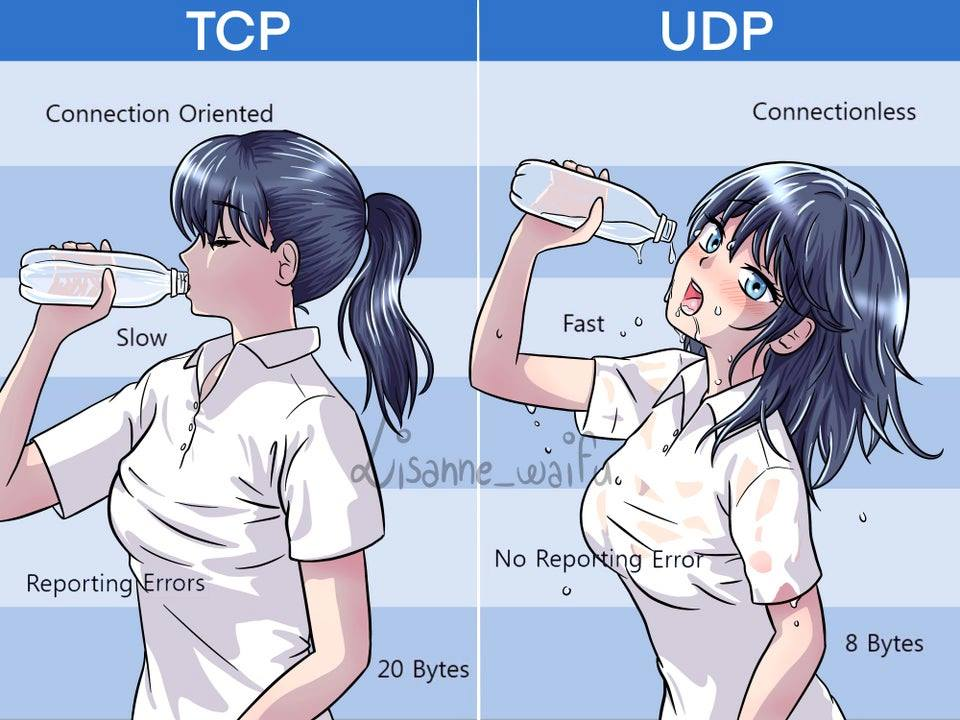
\includegraphics[width=0.55\linewidth]{img/tcp_vs_udp.jpg}
        };
        \end{tikzpicture}%
        \begin{itemize}
            \item  TCP crea una connessione\\prima di trasmettere i messaggi,\\mentre UDP no
            \item TCP consente il recupero e la\\ritrasmissione dei pacchetti persi
            \item TCP trasmette i pacchetti in\\ordine, mentre UDP no
            \item UDP è più veloce di TCP
            \item UDP viene normalmente utilizzato\\per stream video e audio
        \end{itemize}
    \end{frame}
    
    \begin{frame}
        \frametitle{Porte}
        Dato che la comunicazione è process-to-process, vengono utilizzate delle porte per identificare un servizio o un processo.
        \vskip 0.3cm
        Le porte sono suddivise in 3 categorie:
        \begin{itemize}
            \item Well-known ports (0-1023): normalmente utilizzate dai processi di sistema
            \item Registered ports (1024-49151): assegnate da una autorità centrale (IANA), per specifici servizi
            \item Ephemeral ports (49152-65535): porte dinamiche o private non registrate da IANA
        \end{itemize}
    \end{frame}
    
    \begin{frame}
        \frametitle{Porte comuni}
        \begin{table}[]
        \centering
        \begin{tabular}{|l|l|}
        \hline
         Porte &Servizi  \\ \hline
         21 e 22 &File Transfer Protocol  \\ \hline
         22 &SSH  \\ \hline
         25 &Simple Mail Transfer Protocol  \\ \hline
         53 &Domain Name Server  \\ \hline
         80 &HTTP  \\ \hline
         443 &HTTPS  \\ \hline
        \end{tabular}
        \end{table}
    \end{frame}
    
    \begin{frame}
        \frametitle{DNS}
        IL DNS (Domain Name System) è un insieme di gestori di tabella e di indirizzi IP. Il suo compito è quello di attuare corrispondenze tra i nomi dei nodi della rete (host) e gli indirizzi IP; quest'operazione viene detta risoluzione. Il servizio è realizzato tramite un database distribuito, costituito da server DNS.
        \vskip 0.3cm
    
        Ogni organizzazione ha un proprio gestore DNS e coordina le richieste dei suoi utenti.\\
       
        
        Il DNS ha una struttura gerarchica ad albero rovesciato, ed è diviso in domini (com, org, it ecc).\vskip 0.3cm
        
        I domini sono logici e non sono collegati alla rete fisica.
    \end{frame}
    
    \begin{frame}
        \frametitle{DNS ricorsivo}
        \begin{tikzpicture}[overlay,remember picture]
            \node[anchor=south east,xshift=-15pt,yshift=30pt]
              at (current page.south east) {
            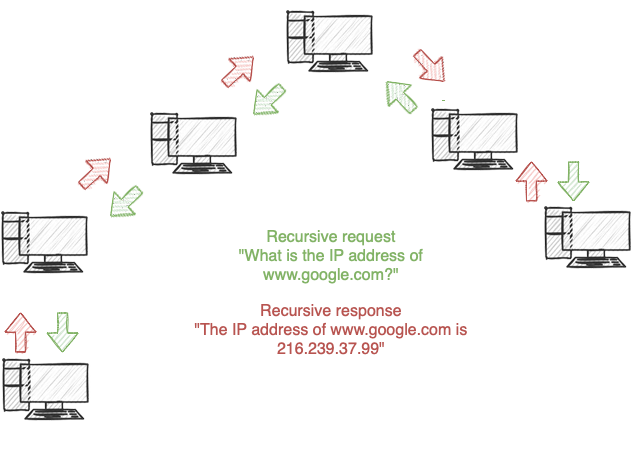
\includegraphics[width=0.55\linewidth]{img/recursive.png}
            };
        \end{tikzpicture}%
        Se il server DNS a cui si è\\ fatta la richiesta è responsabile del\\ dominio, risolve l'indirizzo, altrimenti\\ trasmette la richiesta ad un server\\ DNS di livello superiore e aspetta la\\ risposta per il client.\\ Successivamente il root server inoltra\\ la richiesta al server interessato\\ (passando prima per i server del\\ livello superiore a quello richiesto).\\ Se non viene trovato il server\\ entro un time out si segnala errore.
    \end{frame}
    
    \begin{frame}
        \frametitle{DNS iterativo}
        \begin{tikzpicture}[overlay,remember picture]
            \node[anchor=south east,xshift=-15pt,yshift=30pt]
              at (current page.south east) {
                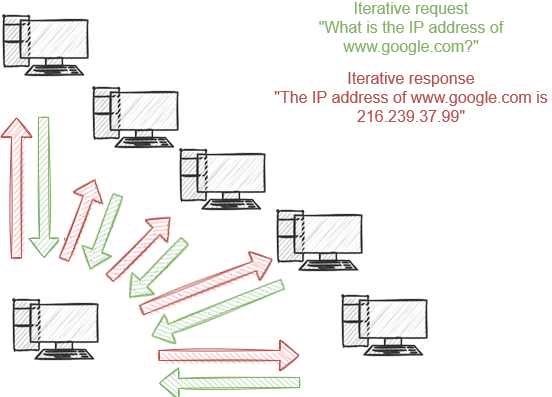
\includegraphics[width=0.55\linewidth]{img/iterative.png}
              };
        \end{tikzpicture}%
        Se il server DNS a cui si è\\ fatta la richiesta è responsabile del\\ dominio, risolve l'indirizzo, altrimenti\\ invia al client il nome del server che\\ secondo lui è in grado di rispondere.
    \end{frame}
    
    \begin{frame}
        \frametitle{Come funziona DNS?}
        \begin{figure}
            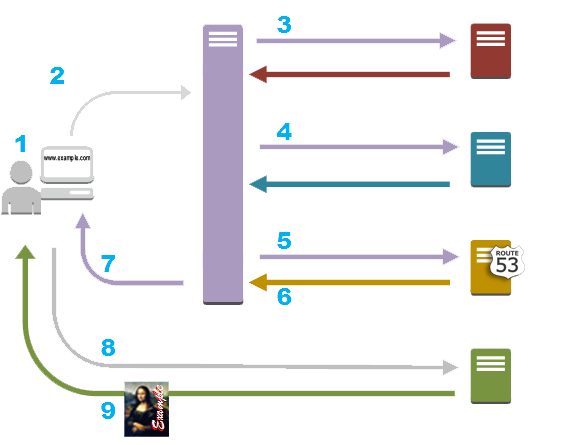
\includegraphics[width=0.6\linewidth]{img/dns_resolver.png}
        \end{figure}
    \end{frame}
    
    \begin{frame}
        \frametitle{DNS rebinding}
        Un attacco DNS rebinding avviene quando un sito web dannoso finge che gli indirizzi IP facciano parte del suo dominio. In questo modo il sito può aggirare i criteri della stessa origine implementati dai browser e visualizzare i dati di tali indirizzi IP.\vskip 0.3cm
        Può verificarsi un attacco DNS rebinding se qualcuno visita un sito web dannoso che identifica l' indirizzo IP locale della vittima, deducendone la struttura della sua rete locale. 
        \\
        Il sito web dannoso potrebbe quindi associare i propri domini all'indirizzo IP locale, inviare richieste ai dispositivi sulla rete e leggere le risposte a tali richieste. 
    \end{frame}
    
    \begin{frame}
        \frametitle{Firewall}
        La funzione di un firewall è quella di proteggere una o più macchine da accessi indesiderati provenienti dall'esterno.
        \\
        Vi possono essere 2 tipologie:
        \begin{itemize}
            \item Packet Filter: posto tra rete locale e Internet, filtra i pacchetti e può scartarli in base a provenienza e destinazione, porta, etc
            \item Proxy Server: filtra i dati sulla base dei protocolli applicativi, non si ferma semplicemente al livello di rete come il packet filter. Tutto il traffico da e verso l'esterno deve passare da esso
        \end{itemize}
    \end{frame}
    
	\startlayoutpage
	\begin{frame}
		\begin{center}
			\Huge Domande?
		\end{center}
	\end{frame}
	\stoplayoutpage
\end{document}
